% Current negative-result edition. Old paper/main.tex and old freezes are unchanged.
\documentclass[10pt]{article}
\usepackage[margin=0.85in]{geometry}
\usepackage{amsmath,amssymb,booktabs,array,longtable,graphicx,hyperref,microtype}
\hypersetup{hidelinks,pdftitle={History dependence without qualified common support},pdfauthor={networkRLCD project}}
\setlength{\emergencystretch}{2em}
\graphicspath{{../../reports/figures/}}
% Rounded existing report values only. No reanalysis or model search.
\newcommand{\NVNinePSNR}{0.508}
\newcommand{\NVNinePSNRLow}{0.077}
\newcommand{\NVNinePSNRHigh}{0.938}
\newcommand{\NVTenDelta}{-14.1}
\newcommand{\NVTenLow}{-22.6}
\newcommand{\NVTenHigh}{-5.5}
\newcommand{\MFiveKampar}{0.20746}
\newcommand{\MFiveKamparLow}{0.09910}
\newcommand{\MFiveKamparHigh}{0.31413}
\newcommand{\MFiveVolga}{0.14750}
\newcommand{\MFiveVolgaLow}{0.09807}
\newcommand{\MFiveVolgaHigh}{0.19353}
\newcommand{\POOneTable}{%
\begin{table}[ht]
\centering\small
\begin{tabular}{lrrrrrr}\toprule
&\multicolumn{3}{c}{Factual BWE MAE (octaves)}&\multicolumn{3}{c}{Synthetic advantage MAE}\\
Family&Persistence&S1&H1&Constant&S1&H1\\\midrule
sawtooth & 0.740 & 0.457 & 0.469 & 0.256 & 0.204 & 0.203\\
square\_wave & 0.684 & 0.413 & 0.421 & 0.251 & 0.200 & 0.199\\
slow\_fade & 0.587 & 0.447 & 0.469 & 0.183 & 0.152 & 0.154\\
feedback\_flap & 0.407 & 0.716 & 0.724 & 0.080 & 0.221 & 0.225\\
\bottomrule\end{tabular}
\caption{PO1 frozen validation values: 72 episodes/family across three fixed fits, six nested decisions/episode. S1 is the fixed-history summary baseline; H1 adds ordered lags. Lower is better. These are simulator results, not native effects.}\label{tab:po1}
\end{table}}

\title{History dependence without qualified common support:\\
Limits of learned native bitrate control}
\author{networkRLCD project\\Retrospective research-decision synthesis}
\date{15 October 2026 --- negative-result edition, evidence through PO1}
\begin{document}
\maketitle

\begin{abstract}
Fine-grained learned bitrate control requires a defensible connection between
sender information, randomized action effects and future delivery risk. We
synthesize frozen native Chromium and simulator studies that did not establish
that connection robustly. A local native study found a positive secondary BWE-by-
action PSNR interaction, but a direct threshold-policy trial reduced timely
delivery by 14.1 percentage points (95\% interval $[-22.6,-5.5]$) relative to
fixed 0.65. An independently sourced replication reversed the descriptive quality
interaction in both measured campaigns but failed registered cell coverage, so
it supplies no population reversal estimate. Subsequent native support studies
failed occupancy or repeatability before their action stages. A qualified
randomized-prefix experiment nevertheless establishes finite-horizon causal
history effects on native BWE, with content/time heterogeneity and no registered
sustained convergence by 36 s. Matching, conditioning and phase-aware rules did
not produce prospectively qualified common state. Available mechanism channels
did not explain residual divergence under their frozen criteria; actual internal
transport timing could not be exposed with both causal freshness and stable
identity. A proposed instrumented browser was never built because resource
admission failed. Finally, a separately preregistered 816-episode simulation
screen failed out-of-family prediction, action-discrimination and useful
uncertainty gates against strong simple baselines. Its native panel remains
unopened. We close the current fine-grained learned-control objective under
these fixture/data assumptions. This is neither a universal impossibility
result nor evidence that all history is irrelevant. We specify the distinct
evidence needed for a new fixture or a different episode-level estimand,
without selecting a successor or fitting another controller.
\end{abstract}

\section{Research question and contribution}
Interactive media must balance source quality, timely delivery and network cost;
these goals are not interchangeable~\cite{rfc8836}. A native sender's reported
bandwidth estimate (BWE) is an output of a transport/encoder feedback system,
not an exogenous measurement of usable capacity. A controller could exploit
observable history only if its action-value and risk claims are identifiable
for the relevant population and survive validation. Good mean prediction in one
regime is insufficient; useful uncertainty must also transport~\cite{ovadia}.

The original networkRLCD program investigated calibrated learned adaptation in
simulation, then native action effects and causal support. This edition changes
the central paper claim to the accumulated negative finding. It does not erase
earlier positive or negative simulator studies, replace their results, or claim
their mechanisms are native WebRTC. Its evidence anchor is commit
\texttt{f109ab2}, the completed PO1 result. All prior tracked artifacts, including
the earlier controller-centric manuscript, are preserved.

The contributions are: (i) a separation of bounded native action evidence from
prospective support failures; (ii) qualified causal history dependence alongside
unsuccessful attempts to obtain useful common state; (iii) a precise distinction
between observability limits and an unattempted instrumented build; and (iv) a
bounded synthetic negative result that requires calibration and supported action
discrimination as well as accuracy. We report a research stopping decision,
not a new bitrate controller or safety certificate.

Earlier simulator studies retain their reported local successes and failures
in the frozen prior edition~\cite{earlier}. They used different representations,
policies and targets; PO1 does not erase those results or supply their native
validation. Passing some synthetic population-panel criteria did not establish
uniform within-family calibration or native control value.

\section{Estimands and what failure means}
\label{sec:estimands}
Let $\mathcal I_t$ contain sender observations, past commands and records
\emph{actually received} by decision time $t$. Let $U_t$ denote unobserved
transport state, $A_t$ a bitrate action and $Y$ a specified future endpoint.
Three questions must remain separate:
\begin{align}
\tau_H(t;S)&=\mathbb E[\log_2 B_t(H_d,S)-\log_2 B_t(H_a,S)],\\
\tau_A(s;\mu)&=\mathbb E_{\mu}[Y(a_1)-Y(a_0)\mid g(\mathcal I_t)=s],\\
V_{\mu}(\pi)-V_{\mu}(\pi_0)&=\mathbb E_{\mu}[Y(\pi)-Y(\pi_0)].
\end{align}
The first is a total effect of randomized early service order $H$ followed by
common input service $S$. The second is a conditional action effect under a
specified history/episode distribution $\mu$. The third is a complete policy
or sequence contrast. A factual predictor
$\mathbb E[B_{t+1:t+h}\mid\mathcal I_t,\text{logging regime}]$ is a fourth,
predictive target; it is not a native counterfactual action value.

Randomized actions can identify local or marginal effects despite hidden
$U_t$, subject to consistency, actual randomization/positivity and the stated
population. Observing every GCC mechanism or finding a stationary Markov state
is not a universal prerequisite for randomized policy inference. Native V9 and
V10 demonstrate that bounded causal contrasts can be estimated in this fixture.
The project's intended \emph{transferable fine-grained conditional value},
however, additionally needs support and a defensible relationship between
the selected observable context and its future response across histories and
sources. That relationship has not qualified. Changing $\mu$ can change the
latent-history mixture even when instantaneous BWE is the same.

We distinguish a contradicted specific superiority claim, an unsuccessful
registered operational recipe, an unestimable comparison after a gate failure,
and a fixture/practical limit. None alone is a theorem that all learned native
control is impossible. Failed support sessions are not treatment outcomes;
zero emitted predictions have unestimable precision. Receiver outcomes left
unopened in support studies are not assigned zero effects.

\section{Evidence handling, sources and technical controls}
\label{sec:evidence}
This is a synthesis of committed result reports and their pinned provenance,
not a meta-analysis or raw-data reanalysis. No captures are restored, no closed
validation representation is searched, no receiver outcome is opened and no
new model is fitted. The evidence ledger binds all cited reports, protocols,
selected storage receipts and manuscript inputs to SHA-256. A preservation audit
checks every file tracked at the evidence anchor. The new edition is separate
so that old scientific freezes remain valid.

Native Chromium outcomes, native responses to controlled synthetic service,
measured-rate replay and simulated outcomes are distinct. Native V9/V10 used
generated content and a controlled schedule; their native telemetry is not a
fluid simulation. V11D crossed licensed source content with four strata nested
in two measured campaigns. V12 used three campaigns. V13's LTE/EVDO bundles
come from one measurement program. M5 onward reuse two licensed clips and
measured-source apparatus; many later common-service plateaus are controlled
inputs. A fresh browser process is a fresh run, not a new independent content
production or network campaign. Measured application-throughput replay is not
a live Internet trial or an observation of every end-to-end queue.

The managed browser policy prohibits nonproxied UDP. Qualified native acquisition
used TURN/TCP without changing that policy. Sender/relay clock markers,
actual-run held-out clock coverage, native initialization, cap/jitter readback,
replay fidelity and cleanup were enforced before admitted analyses. Later
receipt-based features could not use future clock anchors or backdated event
timestamps. Technical qualification is necessary for attribution, but is not
scientific common support. We retain original failures and prospective repairs
as separate studies rather than replacing failed originals.

\section{Native action evidence did not establish transferable value}
\subsection{A local secondary signal and a harmful policy}
Native V9 randomized0.65 versus 1.05 BWE-relative caps at six3s boundaries in 48
sessions, nested in 12 generated-scene seed clusters. Eleven clusters met the
registered state/action counts; one remained in the evidence but outside the
complete-cell analysis. The primary high-minus-low BWE interaction in the150ms
on-time fraction was $-1.8$ percentage points, with an unadjusted95\% $t$ interval
$[-29.4,25.8]$. The secondary PSNR interaction was
$\NVNinePSNR{}$dB $[\NVNinePSNRLow{},\NVNinePSNRHigh{}]$~\cite{v9}.
PSNR is sampled among on-time frames, not common-frame quality under all actions
or human QoE. This supports a local secondary signal under that logging regime,
not a stable state value or policy benefit.

Native V10 tested the direct whole-session implication: use1.05 above the frozen
500 kbps BWE boundary and 0.65 below, versus fixed 0.65. All48 sessions qualified;
two repeats/policy were averaged within each of 12 scene seeds. The threshold
policy's on-time contrast was $\NVTenDelta{}$ percentage points
$[\NVTenLow{},\NVTenHigh{}]$. Overall PSNR was $+0.257$dB $[-0.132,0.646]$.
The fixed threshold's local superiority claim is contradicted~\cite{v10}.
This policy is closed and is not retuned. A positive quality interaction did not
translate into whole-session delivery improvement.

\subsection{Under-covered replication and action stages that never opened}
V11D completed64 qualified native captures from four content groups, four
network-family strata and two measured campaigns. Only9/16 crossed cells had
at least two holds in every state/action bucket; at least 13 were required.
Only seven cells had PSNR in every bucket. Their descriptive PSNR interaction
was $-0.609$dB, with campaign means $-0.419$dB (NordicDat) and $-0.862$dB
(Rome)~\cite{v11d}. Both directions oppose V9, but the coverage gate failed.
We call this a negative, under-covered replication, not an estimate of a
population reversal. No missing bucket is imputed or used to manufacture an
independent campaign sample.

V12 attempted all 24 support originals before randomizing any action. Twenty-three
ordinary captures sealed and one preserved capture failed native media statistics.
Ten passed all gates; none of six cells had complete frozen low/high-BWE support.
The23 ordinary captures passed clocks, transport, replay and cleanup. All48
planned action sessions stayed unrun~\cite{v12}. Capacity-based source hints did
not guarantee native estimator occupancy.

V13 replaced the binary split with a preregistered continuous BWE interaction,
but still required support before actions. All32 originals individually
qualified. Six of 16 content/profile contexts exceeded the0.25-octave fresh-repeat
limit; only one of four cells passed completely. All cells passed profile range
and SD, yet the cross-cell support intersection was empty. Its64 randomized
action sessions remain unrun~\cite{v13}. These failures provide no action-effect
or QoE result. They constrain the design assumptions under which a later effect
would be interpreted.

\section{History is causal; usable common state did not qualify}
\subsection{M5's supported finite-history effect}
M5 qualified 84 original sessions and 42 randomized prefix pairs before its causal
comparison. Within each of two reused contents,21 adjacent pairs received
ascending/descending permutations of the same early service multiset and then
the same measured-source suffix. Actual-run clocks and suffix-exposure checks
passed~\cite{m5}. At18s, descending-minus-ascending mean log2-BWE differences
were $\MFiveKampar{}$octave $[\MFiveKamparLow{},\MFiveKamparHigh{}]$ for Kampar
and $\MFiveVolga{}$ $[\MFiveVolgaLow{},\MFiveVolgaHigh{}]$ for Volga. Both
registered distribution tests reject at local $\alpha=0.025$.

Later signed effects changed direction and neither content satisfied sustained
convergence through 36 s. Thus early service history causally changes later native
BWE in this fixed recipe. This does not establish permanent memory, behavior
beyond the horizon, independent network replication, or a unique mediator.
Holding later service input common does not force identical internal queue,
encoder or estimator trajectories.

\subsection{Matching, conditioning and dynamic-state failures}
M6R qualified 32 originals but only four of six frozen content/landmark strata
met membership coverage. Adding recent encode-time history excluded zero
BWE-only matches; the selected state had exactly the baseline membership.
Conditional future comparisons were therefore not run~\cite{m6r}. This is sparse
overlap and absent matching discrimination at those calipers, not a null causal
history effect. Matching on post-prefix BWE/history also cannot by itself identify
a direct prefix effect or causal mediation.

M7RA's four feasibility originals passed technical gates, but only two reached
the instantaneous target and one met sustained-history membership. Neither
region qualified across histories. Its128-session validation remains
untouched~\cite{m7ra}. A fixed conditioning recipe did not create common state;
similar census means could not replace sustained occupancy.

M8's16 characterization originals under repeated24s controlled-service plateaus
showed strongly asymmetric native dynamics: rise t50 about 7.4--10.2 s and t90
13.3--15.9 s, versus fall t50 about 0.39--0.79 s. At each frozen candidate age,
none of 64 nested plateau occurrences passed future verification under the D1
local-settling rule. No conditioning age was selected~\cite{m8}. These are native
responses of content, encoder and transport to controlled service, not isolated
GCC parameters. The onset search was censored and cannot prove permanent
nonsettling.

M9R prospectively extended observation to a64s common plateau; all eight
instrumentation and 64 validation originals qualified. Instantaneous BWE (B0)
tagged 64 originals and D1 tagged 55, with no future-verified first predictions.
The phase-aware P2 rule emitted no tag, making its positive precision
unestimable. Full four-pair matching coverage fell from42/64 nested strata for
BWE-only to13/64 for the compact history vector, and residual future divergence
remained in some matched contexts~\cite{m9r}. Later observation did not establish
prospectively useful state. It licenses neither another fixed wait nor a
classifier on these closed captures.

\section{Mechanism observability and build practicality}
\subsection{M10R: available counters did not resolve residual divergence}
M10R qualified four instrumentation and eight fresh development originals at
1.414 Mbps common input. It observed acknowledged owned-relay queue/service
counters, native RTCP RTT, RTT-counter detection age, send/cap history and
encoder behavior. No channel met the frozen repeated same-direction contrast
with controls in both contents. Of96 nested contrasts,49 compact-matched and 23
exceeded the0.25-octave future-distance bound. There were 0/400 nested positive
stationary labels, so no stability classifier was fitted~\cite{m10r}.

RTT-counter detection age is not transport-CC generation/arrival age; the owned
relay is one queue, not every queue in the TURN/TCP path. Available contrasts
may be consequences of BWE or shared causes. This assay established neither
causal mediation nor a stationary or prospectively reproducible trajectory
state. Some repeatable moving marginal distributions are insufficient.

\subsection{M11R: real events lacked jointly useful freshness and identity}
Both M11R native capability originals qualified ordinary acquisition. Identified
RTC logs contained actual TCC, delay/loss estimator-update and probe events.
The gate required at least 90\% of each family sender-available within 250 ms,
clock uncertainty at most50ms and stable PC/SSRC/controller attribution. TCC
freshness was1.78\%/1.89\%; BWE-update freshness1.42\%/1.77\%; probe freshness
0/16 and 0/31. First identified export was about 59 s after measurement start,
followed by roughly5s batches~\cite{m11r}.

Verbose target-update lines were fresh but lacked controller identity; a target
emission is not every estimator update. Trace exports supplied no online sender
receipt. No relay/socket/RTT/RTP-burst equivalent proxy qualified. Thus all
required channels qualified in 0/2 originals. Native transport-timing explanations
remain untested in this fixture, not disproved. A record becomes causally usable
at its receipt, not its earlier producer timestamp.

\subsection{IF1: the instrumented alternative was not built}
IF1 specified pinned Chromium/WebRTC hooks, stable identity, nonblocking event
publication and sender-clock receipt. Its formal admission audit found17.7 GB
free disk on a33.8 GB filesystem, below the source's100GB minimum and IF1's
130 GB/16GiB/4-core build requirement; no qualified remote builder or artifact
was available. There were zero compiler attempts, C++ instrumentation patches,
full source checkouts or new native sessions~\cite{if1}. This is a practical
fixture-admission failure. Neither live instrumentability nor instrumented
Chromium's scientific informativeness was tested. Static hook discovery is not
channel qualification, common support or action value.

\section{PO1: three distinct synthetic failures}
\label{sec:po1}
PO1 was preregistered as a cheap necessary-condition screen before a fresh native
factual panel. It uses the existing fluid bottleneck, simplified AckedBwe and
assumed encoder response, not production libwebrtc~\cite{gcc,po1}. Three fits
use384 fitting,144 calibration and 288 held-out validation episodes in total;
validation covers four generator families disjoint from fitting/calibration.
All816 episodes and all binary training/calibration support gates qualified.
Models/calibrators were locked before validation decoding. Six decisions per
episode are nested; uncertainty resamples episodes within fit, not holds.

The fixed 1.05 synthetic logger is distinct from the frozen native fixed 0.65
baseline. At each decision, the feature vector is saved before hindsight
branches compare0.65 for5s with 1.05 for3s then0.65 for2s. A separate factual
branch continues logging1.05 for5s. Only the simulator supplies those action
branches; none is transferred to native data.

S1 uses current values/masks and past3s means, slopes and missing fractions of
BWE, delivered throughput, RTT, requested cap and actual send rate. H1 adds
only ordered1/2/3s samples/masks. These are fixed-penalty linear/logistic models;
there is no recurrent model, state search or learned policy. Baselines include
persistence, trailing mean, clipped trend, train-only constant and instantaneous
linear models as well as S1. Calibration is held out; proper prediction scores
are not themselves control guarantees~\cite{scoring,ovadia}.

\POOneTable

\paragraph{Prediction did not transport robustly.}
H1 improves on persistence/current-value baselines in three families, but its BWE
MAE is worse than S1 in every family. Under feedback-flap H1 error is0.724 versus
persistence0.407,77.8\% worse; S1 also fails there. This is evidence against this
package's robust out-of-family incremental information, not a claim that all
history is irrelevant.
The assay tests a representation/model/logging/calibration package, not the
information-theoretic sufficiency of every possible function of the history.
That limit does not waive the registered stop on complexity escalation.

\paragraph{Action discrimination did not qualify.}
Advantage-MAE gains of H1 over S1 were only 0.19\% and 0.43\% in two families,
below the frozen5\% requirement, with lower bootstrap improvement bounds below
zero and fit-level sign reversals. The other families worsened. Feedback-flap
H1 advantage MAE0.225 versus constant0.080 is179.4\% worse. These are synthetic
action-value prediction errors, not native causal effects or an executed
policy's reward. Local oracle headroom does not ensure that causal observable
history can discriminate actions under shift.

\paragraph{Coverage, calibration and supported uncertainty also failed.}
Nominal90\% sequence intervals use calibration-episode maximum absolute
residuals. H1 BWE full widths are 4.08--5.40 octaves versus maximum 1.0; advantage
widths2.96--3.31 utility units versus maximum 0.50. Aggregate coverage passed its
minimum and within-fit coverage was at least 75\%, but excessive widths fail
usefulness. This empirical cross-family calibration has no distribution-free
OOD guarantee. Every family fails the binary calibration conjunction;
feedback-flap ECE is0.397 for BWE drop and 0.321 for beneficial advantage.
That family's zero unsafe-positive labels cannot establish risk sensitivity.

An offline supported-action assertion requires a positive advantage lower bound,
benefit probability at least 0.90 and unsafe probability at most0.10, with enough
distinct episodes to assess errors. None qualified in any family, versus a
minimum 30 asserted episodes/family. Zero assertions are insufficient supported
discrimination, not demonstrated safety. No learned action was executed. The
registered stop leaves all 64 native factual sessions untouched; there is no PO1
native predictive result~\cite{po1}.

\begin{figure}[p]
\centering
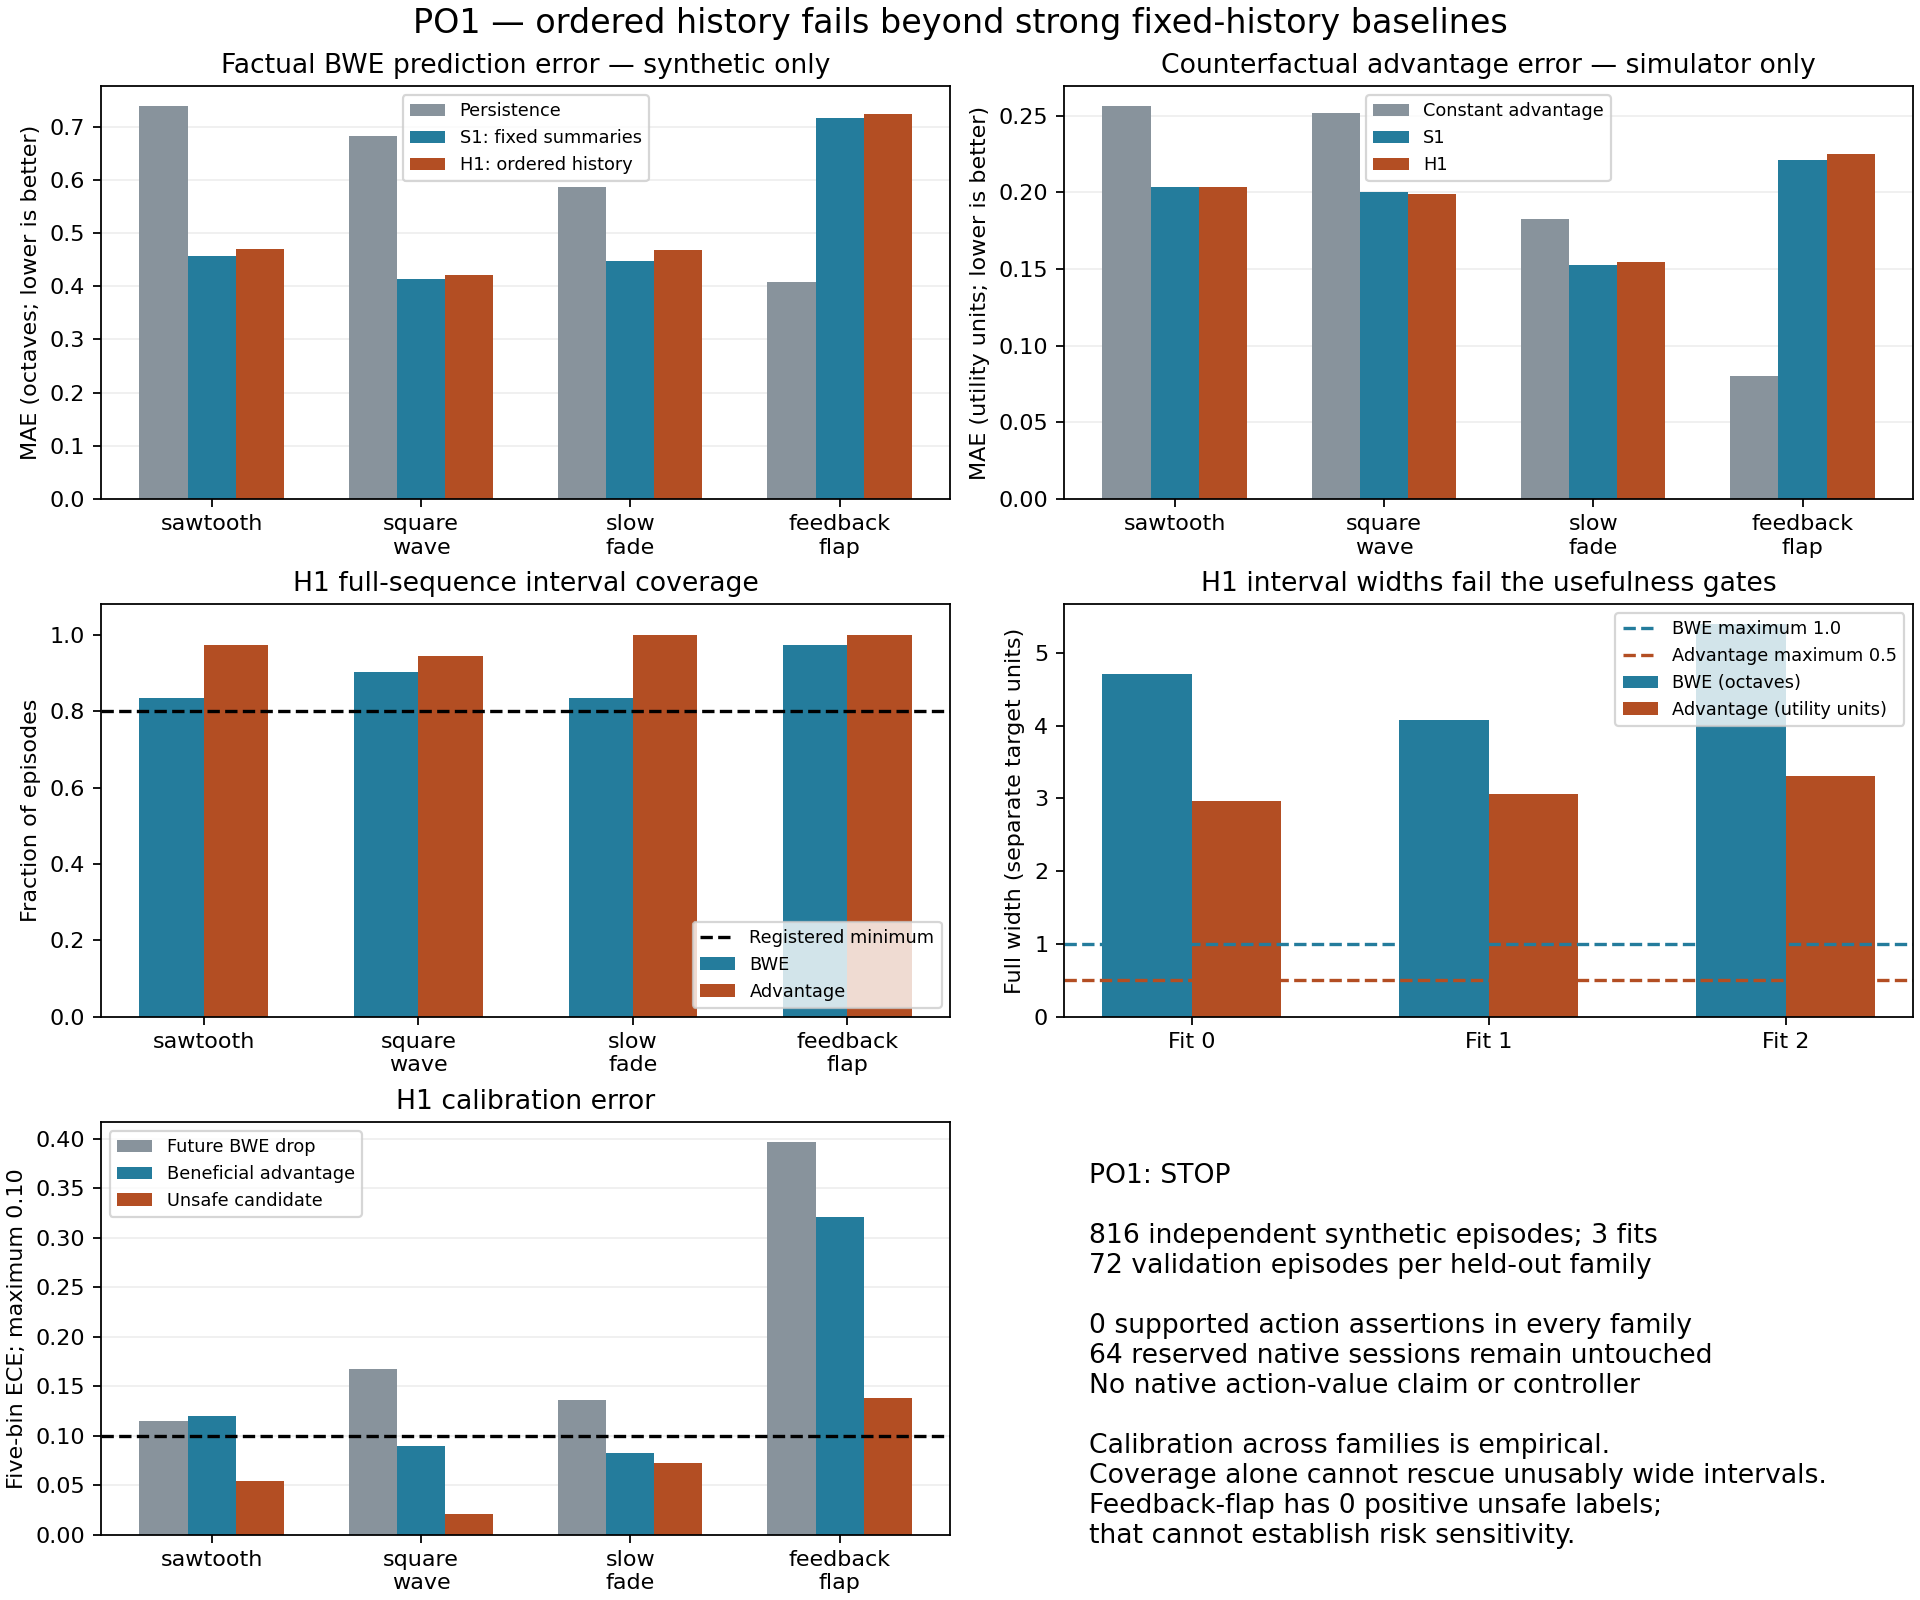
\includegraphics[width=\textwidth]{partial-observability-po1.png}
\caption{Frozen PO1 metrics from its committed report, with no new analysis.
The baseline comparisons, calibration error and interval widths must be read
alongside coverage. All families fail the preregistered conjunction. Families,
fits and decisions are not independent simulator implementations or native
replications.}
\label{fig:po1}
\end{figure}

\section{Research decision and bounded alternatives}
\label{sec:decision}
The active fine-grained learned native-control objective is closed under the
available fixture/data assumptions. No state passed its prospective support
contract; the mechanism route reached an observability boundary; the new fixture
was not admitted; PO1 did not supply robust predictive discrimination or useful
uncertainty. These failures cannot be repaired by pooling sources, relaxing
calipers, opening unused allocations, extending waits, increasing model
complexity or searching closed validation. The PO1 stop remains exact: no history
expansion, retraining with more complex sequence models, calibration/threshold
tuning, native factual panel, controller fit or safe-policy efficacy work from
that representation.

We identify only two conditional changes in premise, neither selected:

\paragraph{A new admitted instrumented fixture.}
An attested builder or verifiable artifact must first make IF1 practical.
Actual transport-feedback, estimator-update, probe and pacer hooks must qualify
identity, causal receipt, freshness, timestamp uncertainty, noninterference and
drop accounting in fresh runs. Fresh technical and observability panels must
precede a new untouched support panel under the original applicable gates.
Only then could a separately preregistered action study test conditional value
and risk over strong fixed 0.65 across independent content/campaigns. Counters
alone neither identify a sufficient state nor justify controller fitting.
No capacity change or build is attempted in this synthesis.

\paragraph{A genuinely different episode/sequence estimand.}
A new research question could randomize complete simple prespecified sequences
at independent episode boundaries under an explicit initial/history-mixture
population, treating within-episode carryover as part of the intervention.
This requires its own permitted fixture, causal/positivity assumptions,
source/campaign clusters, strong fixed 0.65 comparator, risk/precision gates,
stopping rule and fresh data. It cannot reuse PO1's representation or unopened
native allocation, assert washout, or retroactively waive a state gate.
Replicated episode-level benefit would establish that bounded contrast only.
Before fitting an episode-level selector, a separate prospective study would
still need supported sequence-value discrimination and uncertainty under new
source splits. Such evidence would not automatically justify fine-grained
conditional control. No sequence protocol, efficacy panel or learner is
instantiated here.

The default outcome is the present negative-result paper. If neither changed
premise is independently valuable and feasible, the scientifically defensible
decision is to stop, rather than nominate a successor to continue searching.

\section{Limitations and nonclaims}
\label{sec:limits}
These are adaptive research questions with prospectively frozen individual
studies, not one preregistered omnibus experiment. Their sample counts cannot
be summed into a population confidence claim. Generated scenes, reused clips,
directions/windows, repeated landmarks and controlled inputs stay within their
source/campaign clusters. PSNR and 150 ms frame-readback delivery are local
proxies, not human QoE or live deployment safety. Technical qualification does
not establish an empty end-to-end path queue or complete estimator observability.

Specific initial instrumentation failures remain failures: M6's clock
extrapolation, M7's early timers, M7R's launcher, M9's two excessive sample gaps,
M10's cleanup overrun and M11's SSRC0 identity. Prospective repairs use new
captures without changing numerical gates. None is recast as a scientific null
or erased by a successor. IF1 was unattempted at build stage. P2 emitted no tags.
Neither circumstance supplies evidence for a zero mechanism effect.

We have not proved permanent history memory, universal nonsettling, causal
mediation by an internal queue, impossibility of instrumented Chromium, or a
general inability to identify randomized native policy effects. Synthetic
calibration failure is not native calibration failure; no PO1 native prediction
was measured. Conversely, a bounded positive simulator or local native estimate
does not establish broad native control value. This paper documents the missing
evidence rather than replacing it with a stronger claim.

\section{Conclusion}
Native early-service history has a qualified finite-horizon causal effect.
Local randomized action and policy contrasts can be measured, including a
harmful threshold policy. Yet the registered route to reproducible native
conditional value did not qualify. Current diagnostics leave internal timing
unobserved for causal online use; the instrumented build was never attempted;
the compact synthetic history screen failed strong baselines and useful
uncertainty under family shift. Together these results justify stopping the
current fine-grained learned-controller objective under the available fixture
and data assumptions. All frozen evidence and unused panels remain intact.
New measurement capability or a separately justified episode-level question
would require new admission evidence and fresh studies; no controller is fitted
or promoted by this synthesis.

\appendix
\section{Reproducibility and provenance}
The new manuscript and decision document are versioned separately from every
file at\texttt{f109ab2}. The machine-readable claim/source ledger is
\path{data/research-decision-rd1/evidence-ledger.json}; the prior-file freeze is
\path{data/research-decision-rd1/prior-freeze-sha256.json}. The RD1 audit records
summary-only input access, unchanged prior bytes and closed-panel disposition.
The PDF, sources and audit are preserved in a private immutable archive with
fresh object/member size and SHA-256 verification. No licensed media, raw
native session, new receiver endpoint or learned policy is created by RD1.
This retrospective synthesis does not register a new experiment.

\begin{thebibliography}{20}
\bibitem{rfc8836} R. Jesup and Z. Sarker. Congestion Control Requirements for
Interactive Real-Time Media. RFC8836,2021. doi:10.17487/RFC8836.
\bibitem{ovadia} Y. Ovadia et al. Can You Trust Your Model's Uncertainty?
Evaluating Predictive Uncertainty Under Dataset Shift. NeurIPS,2019.
\bibitem{scoring} T. Gneiting and A. E. Raftery. Strictly Proper Scoring Rules,
Prediction, and Estimation. JASA102(477):359--378,2007.
\bibitem{gcc} S. Holmer et al. A Google Congestion Control Algorithm for
Real-Time Communication. IETF draft-ietf-rmcat-gcc-02,2016. Work in progress;
the simulator is not production libwebrtc.
\bibitem{earlier} networkRLCD. RLCD: Calibrated Reinforcement Learning for Safe
Real-Time Media Adaptation. Earlier frozen working manuscript at commit
\texttt{f109ab2}; \path{paper/main.tex}. Historical simulator results retain their
original scope; this negative-result edition supplies the current decision.
\bibitem{v9} networkRLCD. Native clock/action TURN/TCP V9 results. Frozen report.
\path{docs/NATIVE_CLOCK_ACTION_TURN_TCP_V9_RESULTS.md}.
\bibitem{v10} networkRLCD. Native clock/action TURN/TCP V10 results. Frozen report.
\path{docs/NATIVE_CLOCK_ACTION_TURN_TCP_V10_RESULTS.md}.
\bibitem{v11d} networkRLCD. Native clock/action V11D results. Frozen report.
\path{docs/NATIVE_CLOCK_ACTION_TURN_TCP_V11D_RESULTS.md}.
\bibitem{v12} networkRLCD. V12 execution: support qualification failed. Frozen report.
\path{docs/NATIVE_SUPPORT_VALIDATION_V12_RESULTS.md}.
\bibitem{v13} networkRLCD. V13 execution: support failed; action study closed.
\path{docs/NATIVE_CONTINUOUS_VALIDATION_V13_RESULTS.md}.
\bibitem{m5} networkRLCD. M5: qualified instrumentation makes the prefix-history
effect estimable. \path{docs/NATIVE_PREFIX_MEMORY_M5_RESULTS.md}.
\bibitem{m6r} networkRLCD. M6R: history-state common support did not qualify.
\path{docs/NATIVE_HISTORY_STATE_M6R_RESULTS.md}.
\bibitem{m7ra} networkRLCD. M7RA: qualified instrumentation, failed prospective
state creation. \path{docs/NATIVE_STATE_CONDITIONING_M7RA_RESULTS.md}.
\bibitem{m8} networkRLCD. M8: native BWE response to controlled service.
\path{docs/NATIVE_BWE_TRANSIENTS_M8_RESULTS.md}.
\bibitem{m9r} networkRLCD. M9R: prospective phase-aware state and longer-horizon
stability; interpretation and registered residual audit.
\path{docs/NATIVE_PHASE_STATE_M9R_RESULTS.md};
\path{docs/NATIVE_PHASE_STATE_M9R_INTERPRETATION.md}.
\bibitem{m10r} networkRLCD. M10R: fresh causal mechanism observability assay;
qualified observability, mechanism discrimination not established.
\path{docs/NATIVE_MECHANISM_OBSERVABILITY_M10R_RESULTS.md};
\path{docs/NATIVE_MECHANISM_OBSERVABILITY_M10R_INTERPRETATION.md}.
\bibitem{m11r} networkRLCD. M11R: transport-control timing did not qualify for
causal use. \path{docs/NATIVE_TRANSPORT_TIMING_M11R_RESULTS.md}.
\bibitem{if1} networkRLCD. IF1: registered instrumented-fixture plan; build
admission failed. \path{docs/NATIVE_INSTRUMENTED_FIXTURE_IF1_RESULT.md}.
\bibitem{po1} networkRLCD. PO1: bounded observable-history information screen;
result: stop the bounded history-information route. Registration\texttt{d43d407},
result\texttt{f109ab2}.
\path{docs/PARTIAL_OBSERVABILITY_PO1_PLAN.md};
\path{docs/PARTIAL_OBSERVABILITY_PO1_RESULTS.md}.
\end{thebibliography}

\end{document}
